\providecommand{\curso}{Octavo Básico}
\providecommand{\tituloDocumento}{Pauta de corrección}
\providecommand{\subtituloDocumento}{El teorema de Pitágoras}
\documentclass{cdplf-pauta}

\NewDocumentCommand{\sT}{m}{\resizebox{15pt}{!}{$\triangle_{#1}$}}
\NewDocumentCommand{\sC}{m}{\resizebox{15pt}{!}{$\square_{#1}$}}

\def\cuadradoCompleto{%
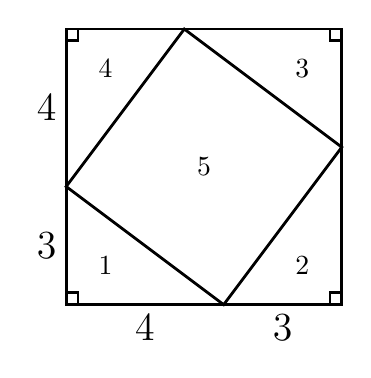
\begin{tikzpicture}[x=0.5cm,y=0.5cm]
    \pgfmathsetmacro{\a}{3};
    \pgfmathsetmacro{\b}{4};

    \draw[line width=1pt] (0,0) rectangle (\a+\b, \a+\b);
    \draw[line width=1pt] (0,\a) -- (\b,0) -- (\a + \b, \b) -- (\a,\a+\b) -- cycle;
    \draw[line width=1pt] (0,0) rectangle +(0.3,0.3);
    \draw[line width=1pt] (\a+\b,\a+\b) rectangle +(-0.3,-0.3);
    \draw[line width=1pt] (0,\a+\b) rectangle +(0.3,-0.3);
    \draw[line width=1pt] (\a+\b,0) rectangle +(-0.3,0.3);

    \node [xshift=0.5cm,yshift=0.5cm] at (0,0) {\sT{1}};
    \node [xshift=-0.5cm,yshift=0.5cm] at (\a+\b,0) {\sT{2}};
    \node [xshift=-0.5cm,yshift=-0.5cm] at (\a+\b,\a+\b) {\sT{3}};
    \node [xshift=0.5cm,yshift=-0.5cm] at (0,\a+\b) {\sT{4}};
    \node [] at (\a/2+\b/2,\a/2+\b/2) {\sC{5}};
    \node at (0,0.5*\a) [left] {\Large 3};
    \node at (0.5*\b,0) [below] {\Large 4};
    \node at (0,\a + 0.5*\b) [left] {\Large 4};
    \node at (\b + 0.5*\a,0) [below] {\Large 3};
\end{tikzpicture}}

\def\tUno{%
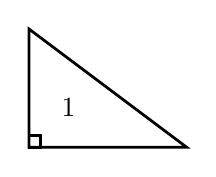
\begin{tikzpicture}[x=1cm,y=1cm,scale=0.5]
    \pgfmathsetmacro{\a}{3};
    \pgfmathsetmacro{\b}{4};
    \draw[line width=1pt] (0,0) -- (\b,0) -- (0,\a) -- cycle;
    \draw[line width=1pt] (0,0) rectangle +(0.3,0.3);
    \node [xshift=0.5cm,yshift=0.5cm] at (0,0) {\sT{1}};
\end{tikzpicture}}
\def\tDos{%
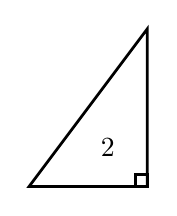
\begin{tikzpicture}[rotate=90,scale=0.5]
    \pgfmathsetmacro{\a}{3};
    \pgfmathsetmacro{\b}{4};
    \draw[line width=1pt] (0,0) -- (\b,0) -- (0,\a) -- cycle;
    \draw[line width=1pt] (0,0) rectangle +(0.3,0.3);
    \node[xshift=-0.5cm,yshift=0.5cm] at (0,0) {\sT{2}};
\end{tikzpicture}}
\def\tTres{%
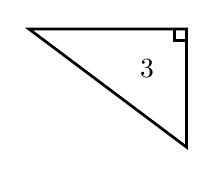
\begin{tikzpicture}[scale=0.5,rotate=180]
    \pgfmathsetmacro{\a}{3};
    \pgfmathsetmacro{\b}{4};
    \draw[line width=1pt] (0,0) -- (\b,0) -- (0,\a) -- cycle;
    \draw[line width=1pt] (0,0) rectangle +(0.3,0.3);
    \node[xshift=-0.5cm,yshift=-0.5cm] at (0,0) {\sT{3}};
\end{tikzpicture}}
\def\tCuatro{%
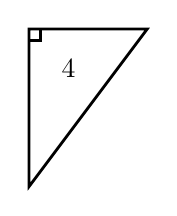
\begin{tikzpicture}[scale=0.5,rotate=270]
    \pgfmathsetmacro{\a}{3};
    \pgfmathsetmacro{\b}{4};
    \draw[line width=1pt] (0,0) -- (\b,0) -- (0,\a) -- cycle;
    \draw[line width=1pt] (0,0) rectangle +(0.3,0.3);
    \node[xshift=0.5cm,yshift=-0.5cm] at (0,0) {\sT{4}};
\end{tikzpicture}}
\def\cChico{%
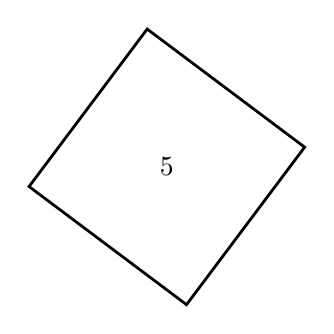
\begin{tikzpicture}[scale=0.5]
    \pgfmathsetmacro{\a}{3};
    \pgfmathsetmacro{\b}{4};
    \draw[line width=1pt] (0,\a) -- (\b,0) -- (\a + \b, \b) -- (\a,\a+\b) -- cycle;
    \node[xshift=0cm] at (\a/2+\b/2,\a/2+\b/2) {\sC{5}};
\end{tikzpicture}
}

\def\figCompleta{%
\begin{tikzpicture}[ampersand replacement=\&,]
    \node (A) {\cuadradoCompleto};
    \node [right=10pt of A.east,anchor=west] (B) {\Huge $=$};
    \node [right=10pt of B.east,anchor=west] (C) {
        \begin{tikzpicture}
            \matrix[matrix of nodes,nodes in empty cells,nodes={minimum height=30pt,minimum width=10pt,anchor=center}] (m) 
                {   \tUno \& {\Huge +} \& \tDos \& {\Huge +} \& \tTres \\
                    \tCuatro \& {\Huge +} \& \cChico  \& \&   \\
                };
            \end{tikzpicture}
    };
\end{tikzpicture} 
}
\usepackage{vwcol}  


\begin{document}
\raggedright
\begin{multicols}{2}

\parte{Resolución de problemas}
\pregunta
\begin{center}
    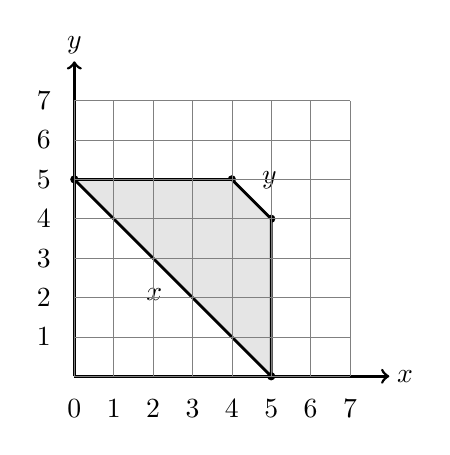
\begin{tikzpicture}[scale=0.5,remember picture]
        \draw[->,shorten >=-5mm,line width=1pt] (0,0) -- (0,7) node[pos=1.2] {$y$};
        \draw[->,shorten >=-5mm,line width=1pt] (0,0) -- (7,0) node[pos=1.2] {$x$};
        \foreach \x in {0,...,7} {
            \node[below=5pt] at (\x,0) {$\x$};
        }
        \foreach \y in {1,...,7} {
            \node[left=5pt] at (0,\y) {$\y$};
        }
        \fill (0,5) circle (3pt);
        \fill (5,0) circle (3pt);
        \fill (4,5) circle (3pt);
        \fill (5,4) circle (3pt);
        \draw[line width=1pt,fill=black!10] (0,5) -- node[below left] {$x$} (5,0) -- (5,4) -- node[above right] {$y$} (4,5) -- cycle;
        \draw[help lines] (0,0) grid (7,7);
        \coordinate (S1) at (3.5,3.5);
    \end{tikzpicture}
\end{center}
El perímetro del trapecio se puede calcular como:
\begin{equation*}
    P = x + 4 + y + 4
\end{equation*}
Donde $x$ e $y$ se pueden encontrar usando el teorema de pitagoras
\begin{equation*}
    x = \sqrt{5^2 + 5^2} \quad \textrm{, y tambien,} \quad y = \sqrt{1^2 + 1^2} \;.
\end{equation*}
Así, el perímetro es:
\begin{equation*}
    P = \sqrt{50} + \sqrt{2} + 8
\end{equation*}
\subsubsection{Área: Método 1}
%\tikz[remember picture,overlay]{\draw[dashed,->] (0,5pt) to[bend right=90,looseness=2] (S1);}
Notemos que el área de cada cuadrado en
la reja es 1 [$\textrm{cm}^2$]. Así, el área del trapecio se puede encontrar 
de la forma:
%\setlength{\abovedisplayskip}{0pt}
%\setlength{\abovedisplayshortskip}{0pt}
\setlength{\belowdisplayskip}{0pt}
\setlength{\belowdisplayshortskip}{0pt}
\begin{align*}
    \textrm{Área}(\raisebox{0pt}{\tikz[]{\draw (0,0) -- ++(45:10pt) -- ++(5pt,0) -- ++(-45:10pt) --cycle;}}) &= \textrm{9 cuadrados} + \textrm{6 mitades}\\
                        &= 9\cdot 1 + 6\cdot 0.5 \\
                        &= 12 \; [\textrm{cm}^2] \\
\end{align*}
\subsubsection{Área: Método 2}
El área del trapecio, también se puede calcular como el área de un 
triángulo menos su punta. Es decir:
\begin{multicols}{2}
        \vspace*{-1cm}
        \begin{tikzpicture}[ampersand replacement=\&,baseline=(current bounding box.south)]
            \matrix[matrix of nodes,nodes={minimum height=2.5cm,anchor=center}] {
                \tikz[scale=0.3]{\draw[fill=black!10] (0,5) -- (5,0) -- (5,4) -- (4,5) -- cycle;} \&
                {\Large $\Huge =$} \&
                \tikz[scale=0.3]{\draw[fill=black!10] (0,5) -- (5,0) -- (5,5) -- (0,5) (4,5) -- (5,4);} \&
                {\Large $\Huge -$} \&
                \tikz[scale=0.3,yshift=4]{\draw[fill=black!10] (4,5) -- (5,5) -- (5,4) -- cycle;} \\
            };
        \end{tikzpicture}
        \columnbreak
%\setlength{\abovedisplayskip}{0pt}
%\setlength{\abovedisplayshortskip}{0pt}
\setlength{\belowdisplayskip}{0pt}
\setlength{\belowdisplayshortskip}{0pt}
\begin{align*}
    \textrm{Área}(\raisebox{0pt}{\tikz[]{\draw (0,0) -- ++(45:10pt) -- ++(5pt,0) -- ++(-45:10pt) --cycle;}}) &= \dfrac{5\cdot 5}{2} - \dfrac{1\cdot 1}{2}\\
                        &= 12.5 - 0.5 \\
                        &= 12 \; [\textrm{cm}^2] \\
\end{align*}
\end{multicols}\vspace*{-1cm}
\pregunta
El cuadrado tiene todos sus lados iguales ($z$) y la diagonal de este forma 
dos triángulos rectángulos
\begin{center}
    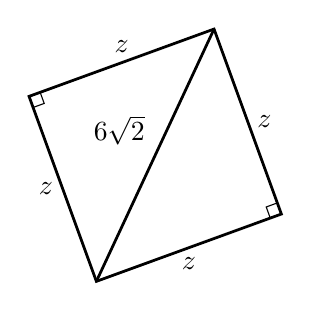
\begin{tikzpicture}[rotate=20,scale=0.5]
        \draw[line width=1pt] (0,0) rectangle (5,5);
        \draw[] (0,5) rectangle +(0.3,-0.3);
        \draw[] (5,0) rectangle +(-0.3,0.3);
        \draw[line width=1pt] (0,0) -- (5,5) node[midway,above left] {$6\sqrt{2}$};
        \node at (0,2.5) [left] {$z$};
        \node at (2.5,5) [above] {$z$};
        \node at (5,2.5) [right] {$z$};
        \node at (2.5,0) [below] {$z$};

    \end{tikzpicture}
\end{center}
\setlength{\belowdisplayskip}{4pt}
\setlength{\belowdisplayshortskip}{4pt}
Usando el teorema de Pitágoras, sabemos que:
\begin{equation*}
    z^2 + z^2 = (6\sqrt{2})^2 = 72
\end{equation*}
Entonces, ¿Qué par de números iguales suman juntos 72? La respuesta 
es 36. Así
\begin{equation*}
    z^2 = 36 \quad \Rightarrow \quad z=6
\end{equation*}
Por lo tanto, el cuadrado es de lado 6. Donde el perímetro es $4\cdot 6=24$ 
y el área es $6\cdot 6 = 36$.
\parte{Demostración del teorema de Pitágoras}

Recordar que: {\slshape ``El área total de la figura es igual a la 
suma de sus partes''}. Es decir:
\resizebox{\linewidth}{!}{\figCompleta}

%
\RenewDocumentCommand{\sT}{m}{\resizebox{10pt}{!}{$\triangle_{#1}$}}
\RenewDocumentCommand{\sC}{m}{\resizebox{10pt}{!}{$\square_{#1}$}}
%
Como el área de la figura completa es $(3+4)\cdot(3+4)=49$ y
los triangulos \sT{1}, \sT{2}, \sT{3} y \sT{4} son iguales y 
de área $(3\cdot 4)/2=6$. Podemos decir que: 
\begin{equation*}
    49 = 6 + 6 + 6 + 6 + \textrm{Área}(\sC{5})
\end{equation*}
Por lo cual, deducimos que el cuadrado \sC{5} tiene área igual a 25 y
sus lados miden 5. Finalmente, hemos mostrado que la hipotenusa
para un triángulo rectángulo de catetos 3 y 4, vale 5.
\end{multicols}
%
\begin{center}
    \tikz{\node [draw,rounded corners,dashed,text width=0.85\linewidth,
        line width=1pt] {Recuerde que esta tarea
    es en preparación para la evaluación de cierre de unidad. Por 
    lo tanto, asegúrese de interiorizar estos contenidos, 
    especialmente si no completo la tarea sol@.};}    
\end{center}
%
\begin{center}
\vspace*{10pt}
\begin{tikzpicture}[ampersand replacement=\&,]
    \node (T) {%
        \begin{tblr}{colspec={X[1,c]X[1]X[8]},width=0.8\linewidth,hline{1,Z} = {1}{-}{}, hline{1,Z} = {2}{-}{}, 
            hlines, cells={valign=m}, row{1} = {bg=black!15}}
            Descuento (puntos)  & Preguntas & Detalle \\
            -2 &  & Desarrollo poco claro o incompleto. No describe procedimientos
            necesarios para solucionar la problemática.\\
            -1 &  & No se llegó a una respuesta, pero muestra dominio de los contenidos involucrados.  \\
            -0.5 & & Pequeño error de cálculo/arrastre.  \\
        \end{tblr}%
    }; 
    \node (A) [right=10pt of T.north east,anchor=north west] {\large\Caja[Puntaje][0.1\linewidth][30pt]};
    \node [below=5pt of A] {\large\Caja[Nota][0.1\linewidth][30pt]};
\end{tikzpicture}
\end{center}

\end{document}